\documentclass[a4paper , final]{ctexart}
\pagestyle{plain}
\everymath{\displaystyle} % 使所有数学公式默认使用行间公式格式

\usepackage{amsmath}
\usepackage[left=2.5cm, right=2.5cm, top=2.5cm, bottom=2.5cm]{geometry}
\usepackage{ifplatform}
\ifwindows
  \setCJKmainfont{SimSun} % 注意:请确保您的系统中已安装宋体 (SimSun) 字体
\else
  \ifmacosx
    \setCJKmainfont{Songti SC} % macOS 上的宋体字体
\fi
\fi
%\usepackage{bookmark}
\usepackage[hidelinks]{hyperref}
\usepackage{graphicx}
\usepackage{subcaption}

\usepackage{enumitem} % 用于自定义列表

% --- 标题格式设置 ---
\usepackage{titlesec}
\titlespacing*{\section}{0pt}{3.5ex plus 1ex minus .2ex}{2.3ex plus .2ex}

\graphicspath{{figures/}} % 图片路径

% --- 核心修改:定义并统一题目环境 ---
\newlist{problems}{enumerate}{1}
\setlist[problems,1]{label=\arabic*., leftmargin=*}

% 环境1:常规题目 (不含图片)
% 使用 \newenvironment 定义新的环境
\newenvironment{problem}[1]{%
  \item #1
  \par
  \vspace{8cm}
}{}

% 环境2:带图片的题目 (已升级)
% #1 (可选): 图片底部距离, 默认 2cm
% #2: 题目文本
% #3: 图片命令
\newenvironment{problemwithfig}[3][2cm]{%
  \item #2
  \par\noindent
  \begin{minipage}[t][8cm][b]{\linewidth}
    \vfill
    \hfill #3
    \par\vspace{#1} % 图片底部的间距由 #1 控制
  \end{minipage}
}{}
% ---------------------------

\title{三角函数}
\date{2025年7月23日}

\begin{document}
\maketitle

\section*{辅助角公式和两角和、倍角公式}

\begin{problems}
  \begin{problem}
        {
            $4\cos{50^\circ}-\tan{40^\circ}=$\underline{\hspace{1.5cm}}.
        }
    \end{problem}
  \begin{problem}
    {
      已知函数 $f(x) = \sin x +2\cos^2\frac{x}{2}$.
      \begin{enumerate}[label=(\arabic*)]
        \item 求 $f(x)$ 的最小正周期及单调递减区间;
        \item 若 $f(\alpha)=\frac94,\alpha\in(\frac{\pi}{4},\frac{\pi}{2})$,求 $\sin\alpha+\sin 2\alpha$ 的值.
      \end{enumerate}
    }
  \end{problem}

  \begin{problem}
    {
      已知角 $\alpha$ 的顶点在坐标原点 $O$,始边与 $x$ 轴的非负半轴重合,将 $\alpha$ 的终边按顺时针方向旋转 $\frac{\pi}{2}$ 后得到角 $\beta$ 的终边,且经过点 $(\frac{2}{\sqrt{5}}, \frac{1}{\sqrt{5}})$.
      \begin{enumerate}[label=(\arabic*)]
        \item 求 $\cos \alpha$ 的值;
        \item 求函数 $f(x) = \cos^2(x-\alpha) + \sin^2(x+\beta)$ 的值域.
      \end{enumerate}
    }
  \end{problem}

  \begin{problem}
    {
      已知函数 $f(x) = \sqrt{3} \sin 2x + 2\cos^2 x - 1$.
      \begin{enumerate}[label=(\arabic*)]
        \item 求函数 $f(x)$ 的单调递减区间;
        \item 将函数 $f(x)$ 分别向左、向右平移 $m(m>0)$ 个单位相应得到 $g(x)$、$h(x)$,且 $\cos m = \frac{\sqrt{3}}{3}  $,求函数 $y = g(x) + h(x)$,$x \in [0, \frac{\pi}{2}]$ 的值域。
      \end{enumerate}
    }
\end{problem}
\newpage
\begin{problem}
  {
    已知函数 $f(x) = \sin x \cdot \cos x - \sin^2 x + \frac{1}{2}$.
    \begin{enumerate}[label=(\arabic*)]
      \item 求函数 $f(x)$ 的单调递增区间;
      \item 若 $f(\alpha) = \frac{2}{3}$,其中 $\alpha \in \left(0, \frac{\pi}{8}\right)$,求 $f\left(\alpha + \frac{\pi}{8}\right)$ 的值.
    \end{enumerate}
  }
\end{problem}

\begin{problem}
  {
    已知函数 $f(x) = \cos x(\sin x + \cos x) - \frac{1}{2}$.
    \begin{enumerate}[label=(\arabic*)]
      \item 求函数 $f(x)$ 的单调增区间;
      \item 求函数 $f(x)$ 在区间 $\left[0, \frac{\pi}{2}\right]$ 上的最大值和最小值.
    \end{enumerate}
  }
\end{problem}

\begin{problem}
  {
    函数 $y = \frac{4\sin x\cos x + 3}{\sin x + \cos x}$,$x \in \left(-\frac{\pi}{4}, \frac{3\pi}{4}\right)$ 的最小值是 \underline{\hspace{3cm}}.
  }
\end{problem}

\begin{problem}
  {
    $\arcsin \frac{\sqrt{14}+3\sqrt{2}}{8}+\arcsin\frac{3}{4}$=\underline{\hspace{3cm}}.
  }
\end{problem}

\begin{problem}
  {
    求函数 $y = 3\sin^2 x - 2\sin 2x + 2\sin x - \cos x, x \in \left[0, \frac{\pi}{2}\right]$ 的值域.
  }
\end{problem}
\end{problems}

\newpage
\section*{对称性、周期性、极值点和单调性}
\begin{problems}
  \begin{problem}
  {
    已知函数 $f(x) = \sin^2\left(x + \frac{\pi}{3}\right) + \frac{1}{2}\cos\left(2x + \frac{\pi}{6}\right)$.
    \begin{enumerate}[label=(\arabic*)]
      \item 求 $f\left(\frac{\pi}{24}\right)$ 的值;
      \item 求函数 $y=f(x)$ 的最小正周期及其单调递增区间.
    \end{enumerate}
  }
\end{problem}

\begin{problem}
  {
    已知函数 $f(x) = \cos^2 x + \cos x \sin\left(x - \frac{\pi}{6}\right)\,(x \in \mathbf{R})$.
    \begin{enumerate}[label=(\arabic*)]
      \item 当 $x \in \left[-\frac{\pi}{4}, \frac{\pi}{6}\right]$ 时,求 $f(x)$ 的值域;
      \item 求 $f(x)$ 在 $[0, \pi]$ 上的增区间.
    \end{enumerate}
  }
\end{problem}
\begin{problem}
        {
            设函数 $f(x) = \cos(\omega x -\frac{\pi}{6})(\omega > 0)$ 的最小正周期为 $\frac{\pi}{5}$,求其对称轴方程.
        }
    \end{problem}

\begin{problem}
  {
    设函数 $f(x) = \frac{\sqrt{3}}{2} - \sqrt{3}\sin^2\omega x - \sin\omega x\cos\omega x\,(\omega > 0)$,且 $y=f(x)$ 的图象的一个对称中心到最近的对称轴的距离为 $\frac{\pi}{4}$.
    \begin{enumerate}[label=(\arabic*)]
      \item 求 $\omega$ 的值;
      \item 求 $f(x)$ 在区间 $\left[\pi, \frac{3\pi}{2}\right]$ 上的最大值和最小值.
    \end{enumerate}
  }
\end{problem}
\end{problems}

\newpage
\section*{三角函数的图像}

\begin{problems}
    \begin{problemwithfig}[5cm]
  {
    已知函数 $f(x) = \sin(\omega x + \varphi)\,(0 < \varphi < \pi)$ 图象上相邻两个最高点的距离为 $\pi$.

    \begin{enumerate}[label=(\arabic*)]
      \item 若 $y=f(x)$ 的图象过点 $(0, \frac{1}{2})$,且部分图象如右图所示,求函数 $f(x)$ 的解析式;
      \item 若函数 $y=f(x)$ 是偶函数,将 $y=f(x)$ 的图象向左平移 $\frac{\pi}{6}$ 个单位长度,得到 $y=g(x)$ 的图象,求函数 $y = 2\left[f\left(\frac{x}{2}\right)\right]^2 + g(x)$ 在 $[0, \frac{\pi}{2}]$ 上的最大值与最小值.
    \end{enumerate}
  }
  {
    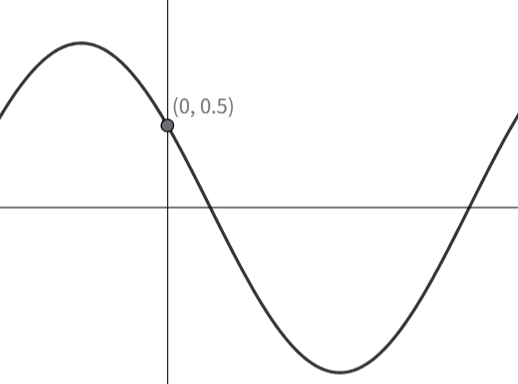
\includegraphics[width=5cm]{Snipaste_2025-07-22_23-03-20.png}
  }
\end{problemwithfig}

\begin{problemwithfig}[5cm]
  {
    已知函数 $f(x) = \frac{\sqrt{3}}{2}\cos^2\frac{\omega x}{2} - \frac{1}{4}\sin(\omega x) - \frac{\sqrt{3}}{4}\,(\omega > 0)$ 的图象如图所示,其中 $A$ 为图象的最高点,$B, C$ 为图象与 $x$ 轴的交点,且 $\triangle ABC$ 为等腰三角形.
    
    \begin{enumerate}[label=(\arabic*)]
      \item 求 $\omega$ 的值及 $f(x)$ 的单调递增区间;
      \item 设 $g(x) = f(x) + f(x+\frac{1}{3})$,求函数 $g(x)$ 在 $[-\frac{1}{2}, \frac{1}{3}]$ 上的最大值及此时 $x$ 的值.
    \end{enumerate}
  }
  {
    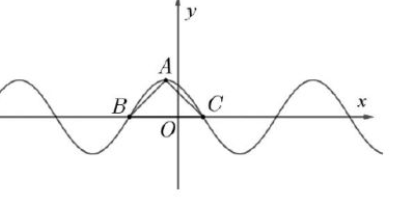
\includegraphics[width=5cm]{Snipaste_2025-07-22_23-11-22.png}
  }
\end{problemwithfig}

\begin{problemwithfig}[5cm]
  {
    已知函数 $f(x) = A\cos(\omega x + \varphi)\,(A > 0, \omega > 0, -\frac{\pi}{2} < \varphi < \frac{\pi}{2})$. $y = f(x)$ 的图象如图所示.
    \begin{enumerate}[label=(\arabic*)]
      \item 求 $f(x)$ 的解析式;
      \item 记 $g(x) = f(x) - \left|x - \frac{5\pi}{6}\right|$,求 $g(x)$ 的最大值.
    \end{enumerate}
  }
  {
    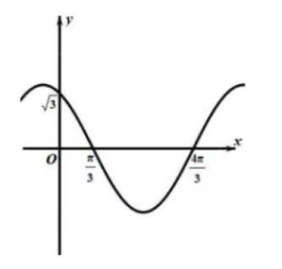
\includegraphics[width=5cm]{Snipaste_2025-07-22_23-32-36.png}
  }
\end{problemwithfig}

\begin{problemwithfig}[5cm]
  {
    已知函数 $f(x) = A\sin(\omega x + \phi)\,(x \in \mathbf{R}, A > 0, \omega > 0, 0 < \phi < \frac{\pi}{2})$ 的图像如图所示;
    \begin{enumerate}[label=(\arabic*)]
      \item 求函数 $f(x)$ 的解析式;
      \item 求函数 $g(x) = f\left(x - \frac{\pi}{12}\right) - f\left(x + \frac{\pi}{12}\right)$ 的单调递增区间.
    \end{enumerate}
  }
  {
    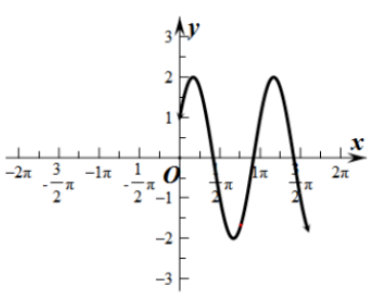
\includegraphics[width=5cm]{Snipaste_2025-07-22_23-35-46.png}
  }
\end{problemwithfig}

\newpage
  \begin{problemwithfig}[5cm]
  {
    已知函数 $f(x) = 4\sin(\omega x + \phi)\,(\omega > 0, 0 < \phi < 2\pi)$ 的部分图像如图所示,$f(x)$ 经过 $(1, 0)$,当 $x = -2$ 时,$f(x)$ 取到最小值.
    \begin{enumerate}[label=(\arabic*)]
      \item 求 $\omega$ 和 $\phi$ 的值;
    \end{enumerate}
  }
  {
    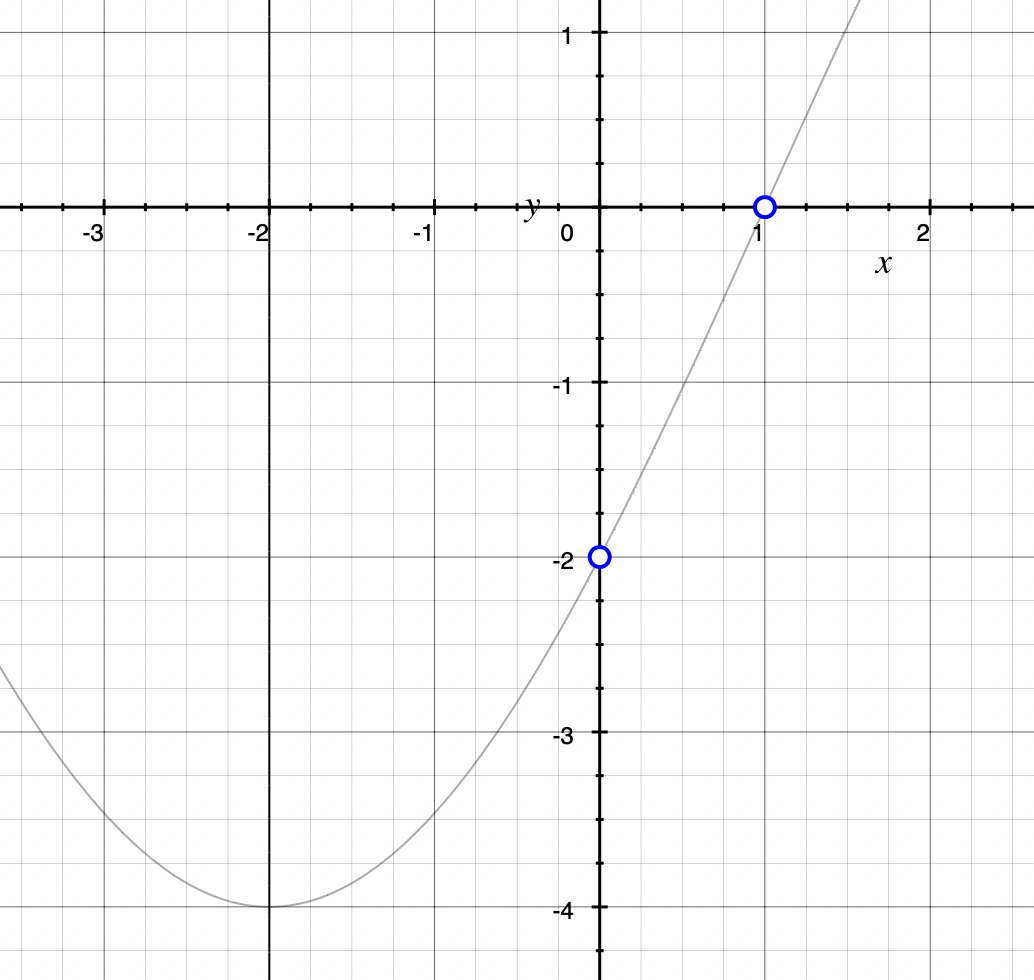
\includegraphics[width=5cm]{Snipaste_2025-07-23_08-50-31.png}
  }
\end{problemwithfig}

\end{problems}


\newpage
\section*{$\omega$ 相关}

\begin{problems}
    \begin{problem}
        {
            已知函数 $f(x) = \sin(\omega x +\frac{\pi}{3})(\omega > 0)$ 在区间 $(0,\pi)$ 内无零点,其图像关于 $x=\frac{2\pi}{3}$ 对称,求 $f(x)$ 的解析式.
        }
    \end{problem}

    \begin{problem}
        {
            已知函数 $f(x) = \sin(\omega x +\frac{\pi}{3})(\omega > 0)$ 的图像关于点 $(\frac{\pi}{3},0)$ 对称,且在 $(\frac{\pi}{4},\frac{\pi}{2})$ 上只有两条对称轴,求 $\omega$ 的值.
        }
    \end{problem}
    
    \begin{problem}
        {
            已知函数 $f(x) = \sin(\omega x +\varphi)(\omega > 0,-\frac{\pi}{2}<\varphi<\frac{\pi}{2}),x=-\frac{\pi}   {4}$ 为 $f(x)$ 的零点,$x=\frac{\pi}{4}$ 为 $y=f(x)$ 的对称轴,且 $f(x)$ 在区间 $\left(\frac{\pi}  {18},\frac{5\pi}{36}\right)$ 上单调,求 $\omega$ 的最大值.
        }
    \end{problem}

    \begin{problem}
        {
            已知函数 $y = \sin(\omega x +\frac{\pi}{6})(\omega > 0)$ 在区间 $(0,\frac{\pi}{2})$ 上有一个最高点和一个最低点,求 $\omega$ 的取值范围.
        }
    \end{problem}
    
    \begin{problem}
        {
            已知函数 $f(x) = 2\cos(\omega x +\frac{\pi}{6})(\omega > 0)$ 在区间 $[-\frac{\pi}{6},\frac{\pi}{3}]$ 上单调递减,且在区间 $[0,\pi]$ 上有且仅有 $1$ 个零点,求 $\omega$ 的取值范围.
        }
    \end{problem}

    \begin{problem}
        {
            已知函数 $f(x) = \cos(\omega x +\varphi)(\omega > 0,-\frac{\pi}{2}<\varphi<0)$,$\left\vert f(-\frac{\pi}{6})\right\vert=1,f(\frac{\pi}{6})=0$,且 $f(x)$ 在区间 $\left(\frac{\pi}{6},\frac{5\pi}{24}\right)$ 上单调,求 $\omega$ 的取值范围.
        }
    \end{problem}

    \begin{problem}
  {
    设函数 $f(x) = \sin\left(\omega x - \frac{\pi}{6}\right) + \sin\left(\omega x - \frac{\pi}{2}\right)$,其中 $0 < \omega < 3$,且 $f\left(\frac{\pi}{6}\right) = 0$.
    \begin{enumerate}[label=(\arabic*)]
      \item 求 $\omega$;
      \item 若 $x \in \left[-\frac{\pi}{12}, \frac{\pi}{3}\right]$,求函数 $g(x) = f^2(x) - f(x) + 1$ 的最大值.
    \end{enumerate}
  }


\end{problem}
\end{problems}

\newpage
\section*{解三角形}
\begin{problems}
  \begin{problem}
  {
    已知在 $\triangle ABC$ 中,角 $A, B, C$ 的对边分别为 $a, b, c$,且 $a\sin B - \sqrt{3}b\cos A = 0$.
    \begin{enumerate}[label=(\arabic*)]
      \item 求角 $A$ 的大小;
      \item 求 $2\cos A + 2\cos B + \cos C$ 的取值范围.
    \end{enumerate}
  }
\end{problem}

\begin{problem}
  {
    在锐角 $\triangle ABC$ 中,角 $A, B, C$ 所对的边分别是 $a, b, c$,$b^2 + c^2 - a^2 = 2bc\sin\left(A + \frac{\pi}{6}\right)$.
    \begin{enumerate}[label=(\Roman*)]
      \item 求角 $A$ 的大小;
      \item 求 $\sin B \cdot \cos C$ 的取值范围.
    \end{enumerate}
  }
\end{problem}

\begin{problem}
  {
    在 $\triangle ABC$ 中,内角 $A,B,C$ 所对应的边分别为 $a,b,c$ 且满足 $a\cos C +c\cos A - 2b\sin B = 0$.
    \begin{enumerate}[label=(\arabic*)]
      \item 求角 $B$ 的大小;
      \item 若 $B$ 为锐角,$\sin A = \frac{\sqrt{6}-\sqrt{2}}{4}$,$BC$ 边上的中线 $AD = \sqrt{7}$,求 $\triangle ABC$ 的面积.
    \end{enumerate}
  }
\end{problem}
\end{problems}

\end{document}